%TODO: CORREGIR COMANDOS PARA QUE SE VEAN CON VERB
%TODO: INTENTAR QUITAR LA MORRAYA QUE NO SIRVA
%TODO: INTENTAR NO REPETIR TANTAS COSAS EN EL EJERCICIO 3
%TODO: REVISAR DOCUMENTO PARA FALLOS ORTOGRAFICOS/GRAMATICALES
\documentclass{article}
\usepackage[utf8]{inputenc}
\usepackage[spanish]{babel}
\usepackage{graphicx, graphics, float, hyperref}
\usepackage{listings, subcaption}
\usepackage[a4paper, total={6in, 10in}]{geometry}

\title{SSO Práctica 4 Sesión 1}
\author{Andrés Merlo Trujillo}
\date{}
\hypersetup{
    colorlinks=true,
    linkcolor=black,
}

\begin{document}

\maketitle

\tableofcontents

\newpage
%\addcontentsline{toc}{section}{Ejercicio 1}
%\section*{Ejercicio 1}
%\begin{figure}[H]
%    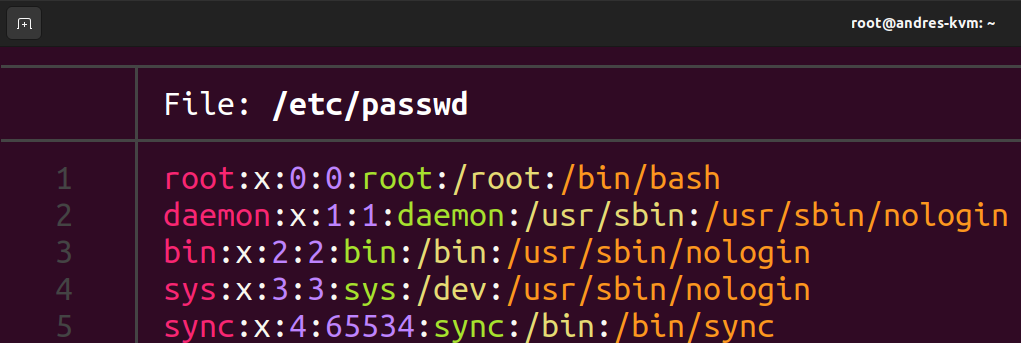
\includegraphics[width=\textwidth]{imagenes/passwdfile.png}
%    \caption{Ejemplo de entradas en el archivo.}
%\end{figure}

\addcontentsline{toc}{section}{Ejercicio 1}
\section*{Ejercicio 1}

Debido a que le pendrive que tengo es muy lento (usa USB 2.0), voy a crear una particion de 1 GB con el sistema de archivos ext4.

Y ahora a modo de realismo, voy a copiar las imagenes usadas durante estas practicas y un archivo dentro de la carpeta ``mis trabajos'' denominado ``amenaza.txt'' con una frase que amenace.

%Foto de la carpeta con archivos y del archivo amenaza

A continuacion elimino esse archivo y desmonto el disco para suponer que he recibido el pendrive asi y para que no pueda realizarle mas modificaciones.

Ahora voy a seguir los pasos indicados en el guion de practicas, por tanto, lo primero que hay que hacer es obtener la estructura interna de particiones con la orden \verb|fdisk -l /dev/sdX > fdisk.disco1| siendo la X la letra asignada al disco, en mi caso es a. (se puede comprobar con la orden \verb|fdisk -l| o \verb|lsblk|).

%foto de la salida del comando

Lo siguiente que hay que hacer es crear una imagen forense del disco para evitar invalidar el contenido del pendrive y trabajar de forma segura sobre una copia. Esto se realiza mediante la orden \verb|dd if=/dev/sda1 of=imagen.disco1 bs=512|.

%salida de dd

Ahora es necesario poner la imagen del disco a solo lectura con la orden \verb|chmod 444 imagen.disco1|.

El siguiente paso, que es copiar la imagen a otro disco no es necesario, ya que se puede trabajar directamente sobre la imagen como explicare a continuacion. Ahora se debe montar la imagen con la orden \verb|mount imagen.disco1 /mnt -o noexec,loop|, y al hacer \verb|lsblk -f| se puede ver que está montado correctamente.

%foto de la salida de lsblk
%caption{Se puede ver que el nombre que tiene es \texttt{loop2} y que se ha montado correctamente en el punto de montaje indicado.}

Ahora es necesario verficar la integridad de los datos del pendrive antes y despues de completar el analisis, para ello se usa la orden \verb|sha1sum /dev/sda1 > SHA.disco1|.

%foto de sha1sum

Y ahora, voy a realizar lo mismo, pero sobre cada archivo. En este caso se debe hacer sobre la imagen porque al montar el pendrive puede darse el caso de que el hash cambie. Para ello, desde la raiz de la imagen montada, se debe hacer con la orden \verb|find . -type f -exec sha1sum {} \; > SHA.listaArchivos|.

%salida del comando con bat

Y se puede realizar la verficiacion con la orden \verb|sha1sum -c ~/SHA.listaArchivos| (se debe estar dentro de la raiz de la imagen)

%salida del comando.

Ahora se puede proceder con seguridad a encontrar el archivo eliminado anteriormente. Para ello, es necesario crear un fichero con las palabras claves mas probables que se encuentren. El fichero tiene la siguiente forma:

%slaida

Ahora con la orden \verb|grep -aibf palabrasClave imagen.disco1 > aciertos.txt| se puede realizar la busqeuda en la imagen:

%salida en aciertos.txt

Como se puede ver, aparece la frase ``Esto es una amenaza, si no nos da algo de dinero publicamos el contenido de su pendr...'', indicando que ha habido una amenaza.

Por ultimo, para asegurarse, se puede usar el comando \texttt{xxd -s 299892684 imagen.disco1 | less} para verlo en la propia imagen:

%salida del comando

Y efectivamente, aqui tamvien aparece.

\addcontentsline{toc}{section}{Ejercicio 2}
\section*{Ejercicio 2}

(NOTA: debido a la lentitud del pendrive que tengo, he decidido usar un pendrive de menor capacidad y con USB 3.0, va a tener exactamente los mismos pasos aplicados que el ejercicios 1, aunque no tendrá el mismo hash seguira produciendo la misma salida.)

EN esta parte es necesario utilizar la herramienta ``GuyMager'' para obtener una imagen forense del mismo pendrive. POr tanto, se descarga el programa mediante \verb|apt| y se abre.

%foto de inicio.

Y se pulsa con click derecho en el dispositivo que se quiera realizar la imagen, en mi caso \verb|/dev/sda|, y le damos a ``Acquire image''.

%ventana nueva

Y ahora simplemente rellenamos los campos que se piden y al final quedan asi:

%foto de esto relleno

Por ultimo, es necesario darle a ``Start'' para que comience el proceso.

%foto del progreso
%caption{Progreso de creacion de imagen forense.}

Al finalizar, se puede ver que ha generado varios trozos de la imagen del pendrive.

%foto

\addcontentsline{toc}{section}{Ejercicio 3}
\section*{Ejercicio 3}

Para este ejercicio es necesario tener instalado ``TheSleuthKit'' y ``Autopsy''. Una vez instalado, es necesario ejecutar la siguiente orden: \verb|sudo autopsy| e irse a la URL \verb|http://localhost:9999/autopsy|.

%imagen inicial

\addcontentsline{toc}{subsection}{Apartado A}
\subsection*{Apartado A}
Una vez lanzado el servidor, es necesargio crear un caso dandole al boton ``NEW CASE''. Dentro del mismo rellenamos los datos que se piden:

%foto de los datos rellenados

Y despues se debe crear un host para este caso, para ello se le da al obton ``ADD HOST'' y se rellenan los datos.

%foto de esto relleno

A continuacion, es necesario añadir la imagen creada con la herramienta ``GuyMager'', para ello, se le da al boton ``ADD IMAGE'' y luego a ``ADD IMAGE FILE''. Despues debemos rellenar la ubicacion de los fragmentos de la imagen utilizando el wildcard ``*'' para indicarle que coja todos los fragmentos.

%fotos dfe las tres pantalals

Finalmente se le da al boton ``ADD'' para que se añadan las imagenes y aparece una pantalla donde se indica las imagenes añadidas junto con algunos detalles (enalce ``details'').



\end{document}
